Agora que estudamos a dinâmica molecular e conseguimos atingir observar o que as velocidades 
seguem distribuições de Maxwell-Boltzman, queremos impor uma dinâmica específica sobre o 
gás 2D. 
Nesse caso queremos observar a cristalização de moleculas, e para isso consideramos uma caixa 
de tamanho $L=4$ com $N = 16$ partículas, ou seja, a densidade nesse caso é $\sigma = 1$, o passo 
foi $\Delta t = 0.005$ e a velocidade inicial de teste $v_0 = 1$. 
No entanto, para essa velocidade não foi possível observar a cristalização acontecendo nos diferentes regimes
de temo desejados, por isso foi necessário diminuir a velocidade inicial $v_0$ para 
$v_0 = 0.2$. Isso condiz com um sistema à baixa temperaturas de alta densidade. 

Como pode ver abaixo (\ref{fig:posicoes-finais-e}) correspondem à cristalização das moléculas. 
Da esquerda para a direita temos o ``rastro'' das partículas nos temos $0 \leq t \leq 0.1$, $0.2 \leq t \leq 0.4$ e 
por fim $13 \leq t \leq 16$. Foram consideradas as posições em intervalos de $ 10 \Delta t$. 

\begin{figure}[h!]
    \centering
    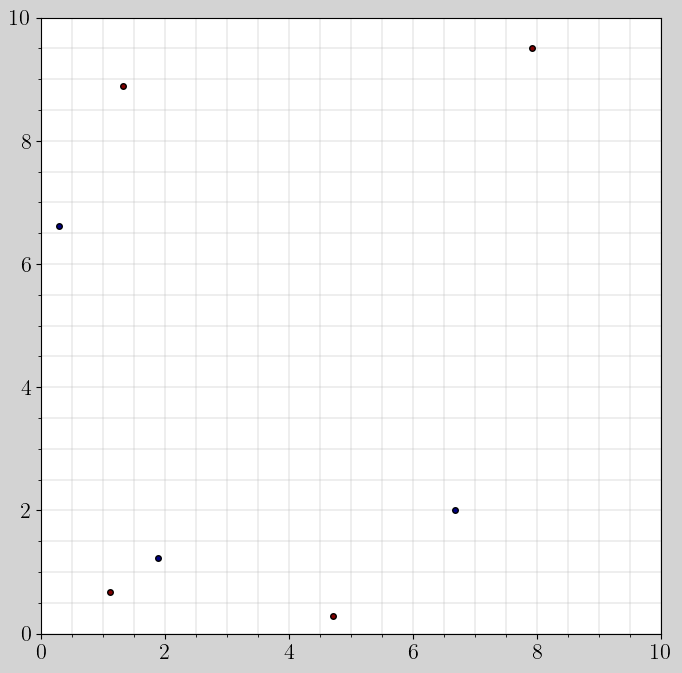
\includegraphics[width=0.95\linewidth]{tarefa-E/posicoes-finais.png}
    \caption{Etapas da cristalização das moléculas.}
    \label{fig:posicoes-finais-e}
\end{figure}


Além desse gráfico foi construido um vídeo para essa tarefa. Esse é um pouco mais longo que os anteriores\footnote{E espero que consiga subir ele para o basalto.}
mas observando apenas os segundos finais dele podemos notar que as partículas permanecem quase presas em uma determinada região nas proximidades da 
do ponto de cristalização. É possível até perceber a estrutura triangular com a qual as partículas se movimentam em torno dos vizinhos. 

\subsection*{Implementação - Simulação E}
\begin{minted}{fortran}

      ! TAREFA E 
      implicit real*8(a-h, o-y)
      parameter (pi = acos(-1.e0))
      dimension r_prev(20, 2)
      dimension r_curr(20, 2)
      dimension r_next(20, 2)
      dimension v(20, 2)
      dimension acc(2)
      dimension r(20, 20)

      open(unit=75, file="saidas/tarefa-E/parametros.dat")
      open(unit=76, file="saidas/tarefa-E/posicoes-iniciais.dat")
      open(unit=77, file="saidas/tarefa-E/evolucao-posicoes-1.dat")
      open(unit=78, file="saidas/tarefa-E/evolucao-posicoes-2.dat")
      open(unit=79, file="saidas/tarefa-E/evolucao-posicoes-3.dat")

      ! Reset variables: 
      r_prev = 0
      r_curr = 0
      r_next = 0
      v = 0

      L = 4
      rL = 4d0
      N = 16
      dt = 5e-3

      v0 = 0.2

      write(75, *) N, L, v0, dt 
      close(75)

      ! Initialize particles 

      n_cols = ceiling(sqrt(N*1d0))
      n_rows = ceiling((N*1d0)/(n_cols*1d0)) 
      
      ! Spacing 1/4 
      x_spacing = L/(1d0*n_cols)
      y_spacing = L/(1d0*n_rows)
      spacing = min(x_spacing, y_spacing)/4.0 
      
      ! Centering in the grid
      x_offset = x_spacing / 2.0 
      y_offset = y_spacing / 2.0
      
      call srand(3512341)

      k = 1 
      do j = 1, n_rows 
            do i = 1, n_cols 
                  r_curr(k, 1) = (i-1)*x_spacing+x_offset
                  r_curr(k, 2) = (j-1)*y_spacing+y_offset
                  
                  r_curr(k, 1) = r_curr(k,1)+(rand())*spacing
                  r_curr(k, 2) = r_curr(k,2)+(rand())*spacing
                  
                  theta = 2*pi*rand()
                  
                  v(k, 1) = v0*cos(theta)
                  v(k, 2) = v0*sin(theta)
                  
                  r_prev(k, 1) = r_curr(k, 1) - v(k, 1) * dt 
                  r_prev(k, 2) = r_curr(k, 2) - v(k, 2) * dt 
                  k=k+1
            end do 
      end do

      do i = 1, N 
            write(76, *) r_curr(i, 1), r_curr(i, 2)
      end do 
      close(76)

      ! Dynamics 
      do k = 1, 3200 
            t = k * dt 
            acc(1) = 0d0 
            acc(2) = 0d0
            do i = 1, N 
                  acc(1) = 0d0 
                  acc(2) = 0d0
                  do j = 1, N 
                        if(i /= j) then
                        call compute_acc(N,i,j,L,r_curr,acc, r)
                        end if
                  end do 
                  ! UPDATE POSITIONS
                  r_next(i,1) = 2*r_curr(i,1)-r_prev(i,1)+acc(1)*(dt**2)
                  r_next(i,2) = 2*r_curr(i,2)-r_prev(i,2)+acc(2)*(dt**2) 

                  ! APPLY PBC
                  r_next(i,1) = mod(r_next(i,1)+rL, rL)
                  r_next(i,2) = mod(r_next(i,2)+rL, rL)

                  delta_r_x = delta_pbc(r_next(i,1),r_prev(i,1),L)
                  delta_r_y = delta_pbc(r_next(i,2),r_prev(i,2),L)

                  ! UPDATE VELOCITIES using adjusted displacements
                  v(i, 1) = delta_r_x / (2 * dt)
                  v(i, 2) = delta_r_y / (2 * dt)
            end do
            r_prev(:, 1) = r_curr(:, 1)
            r_prev(:, 2) = r_curr(:, 2)
            
            r_curr(:, 1) = r_next(:, 1)
            r_curr(:, 2) = r_next(:, 2)

            if(k < 21) then 
                  do i = 1, N 
                        write(77,*) k, r_curr(i,1),r_curr(i,2)
                  end do
            else if (k > 40 .and. k < 81 .and. mod(k,3)==0) then 
                  do i = 1, N 
                        write(78,*) k, r_curr(i,1),r_curr(i,2)
                  end do
            else if (k > 2600 .and. k < 3200 .and. mod(k,10)==0) then 
                  do i = 1, N 
                        write(79,*) k, r_curr(i,1),r_curr(i,2)
                  end do
            end if 
      end do 
      close(77)
      close(78)
      close(79)
      end
      function delta_pbc(r_next, r_prev,L)
            implicit real*8(a-h, o-y)
            delta_pbc = r_next - r_prev
            delta_pbc = delta_pbc - L * nint(delta_pbc / L)
      end function delta_pbc
      ! Updates acceleration a = ax, ay 
      ! between particle i and all others
      subroutine compute_acc(N,i,j,L,r_curr,acc, r)
            implicit real*8(a-h, o-y)
            dimension r_curr(20, 2)
            dimension acc(2)
            dimension r(20, 20)
            epsilon = 1e-3

            dx = r_curr(i, 1) - r_curr(j, 1)
            dy = r_curr(i, 2) - r_curr(j, 2)

            dx = dx - L * nint(dx / L)
            dy = dy - L * nint(dy / L)

            r_ij = sqrt(dx**2 + dy**2)
            
            r(i, j) = r_ij 
            r(j, i) = r_ij

            if(r_ij > epsilon .and. r_ij <= 3d0) then 
                  F = 24.0 * (2d0/r_ij**13 - 1d0/r_ij**7)
                  acc(1) = acc(1) + F * dx / r_ij 
                  acc(2) = acc(2) + F * dy / r_ij
            end if 
      end subroutine compute_acc

      subroutine compute_energy(N, L, v, r_curr, E, r)
            implicit real*8(a-h, o-y)
            dimension v(20, 2)
            dimension r_curr(20, 2)
            dimension r(20, 20)
            
            epsilon = 1e-3
            Tk = 0d0
            do i = 1, N
                Tk = Tk + 0.5 * (v(i, 1)**2 + v(i, 2)**2)
            end do
            U = 0d0
            do i = 1, N
              do j = i + 1, N
                  r_ij = r(i, j)

                  if (r_ij > epsilon .and. r_ij <= 3d0) then
                      U = U + 4 * (r_ij**(-12) - r_ij**(-6))
                  end if
              end do
            end do
            E = Tk + U
      end subroutine
\end{minted}
\clearpage 